\chapter{DNN Input Variables LO to NLO Reweighting}
\label{sec:DNN-Input-Variables-LO_NLO_Weight_Validation}

This section contains ratio plots for each Semi-Leptonic DNN input variable between the sum of 12 LO Benchmarks plus the SM LO point, and the 2017 SM at NLO sample.
The LO samples all have LO to NLO reweighting applied as described in Section \ref{sec:EFT_Description}. There is slight disagreement observed, indicating the network 
is suboptimal, but because these events are only used for training there is no bias introduced in the analysis from any disagreement in these ratios. In addition,
the amount of disagreement observed is not expected to have a detrimental effect on the performance of the network. 

\newpage 

\begin{figure}[h!]
    \setcounter{subfigure}{0}
    \centering
    \subfloat[$m_{jj}$]{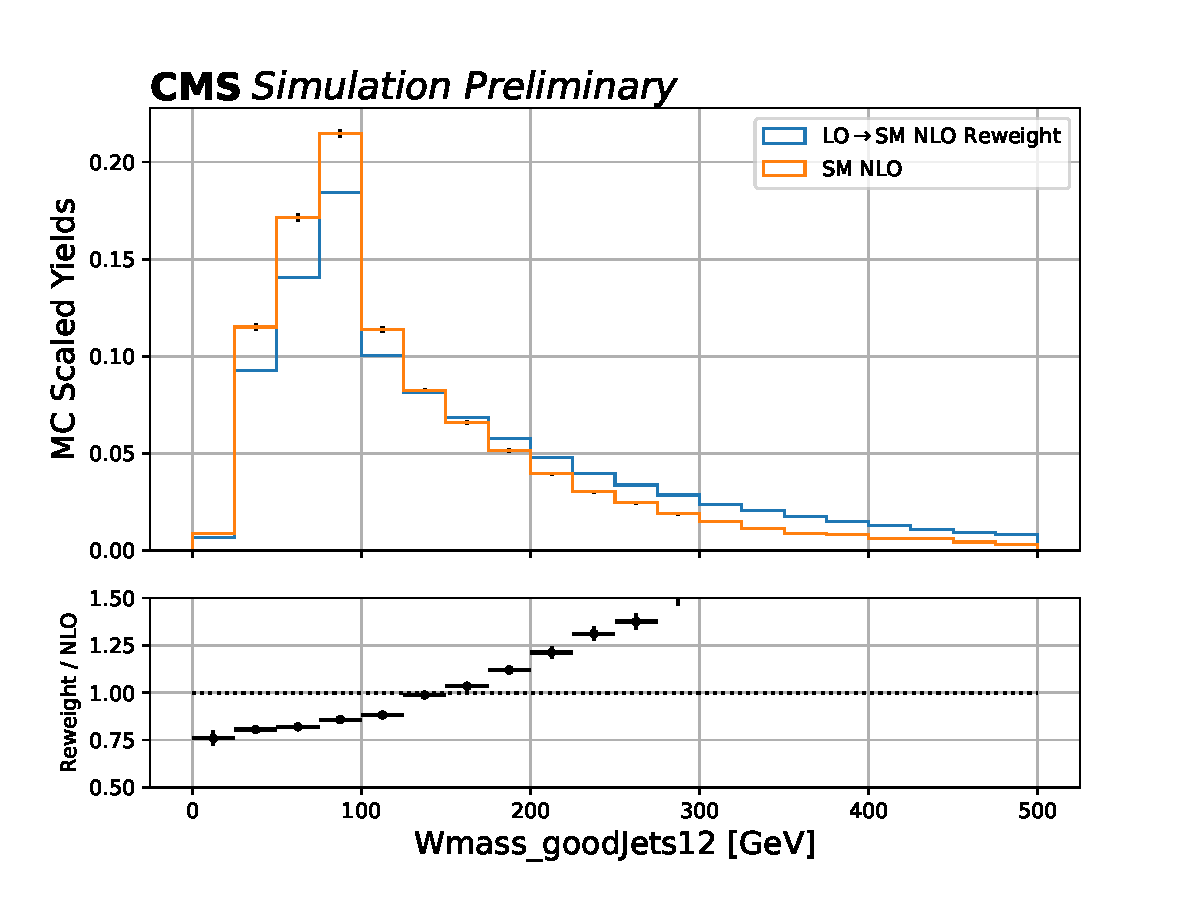
\includegraphics[width=0.4\textwidth]{Sections/HHWWgg/images/DNN/LO_NLO_Reweight_Distributions/Wmass_goodJets12.pdf}}
    \qquad
    \subfloat[Leading Jet $p_{T}$]{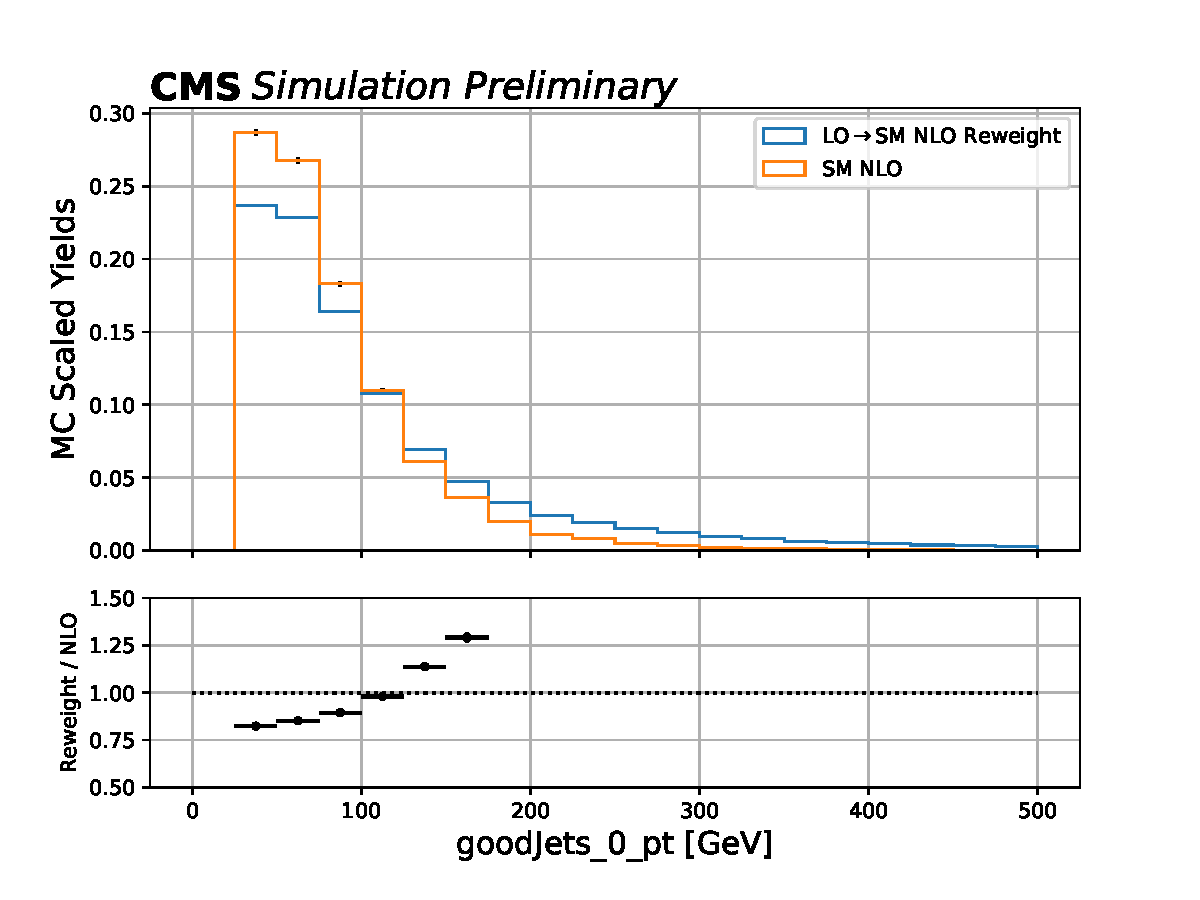
\includegraphics[width=0.4\textwidth]{Sections/HHWWgg/images/DNN/LO_NLO_Reweight_Distributions/goodJets_0_pt.pdf}}
    \caption{Invariant mass of the two leading jets, leading jet \pt}
\end{figure}

\begin{figure}[h!]
    \setcounter{subfigure}{0}
    \centering
    \subfloat[Leading jet Energy]{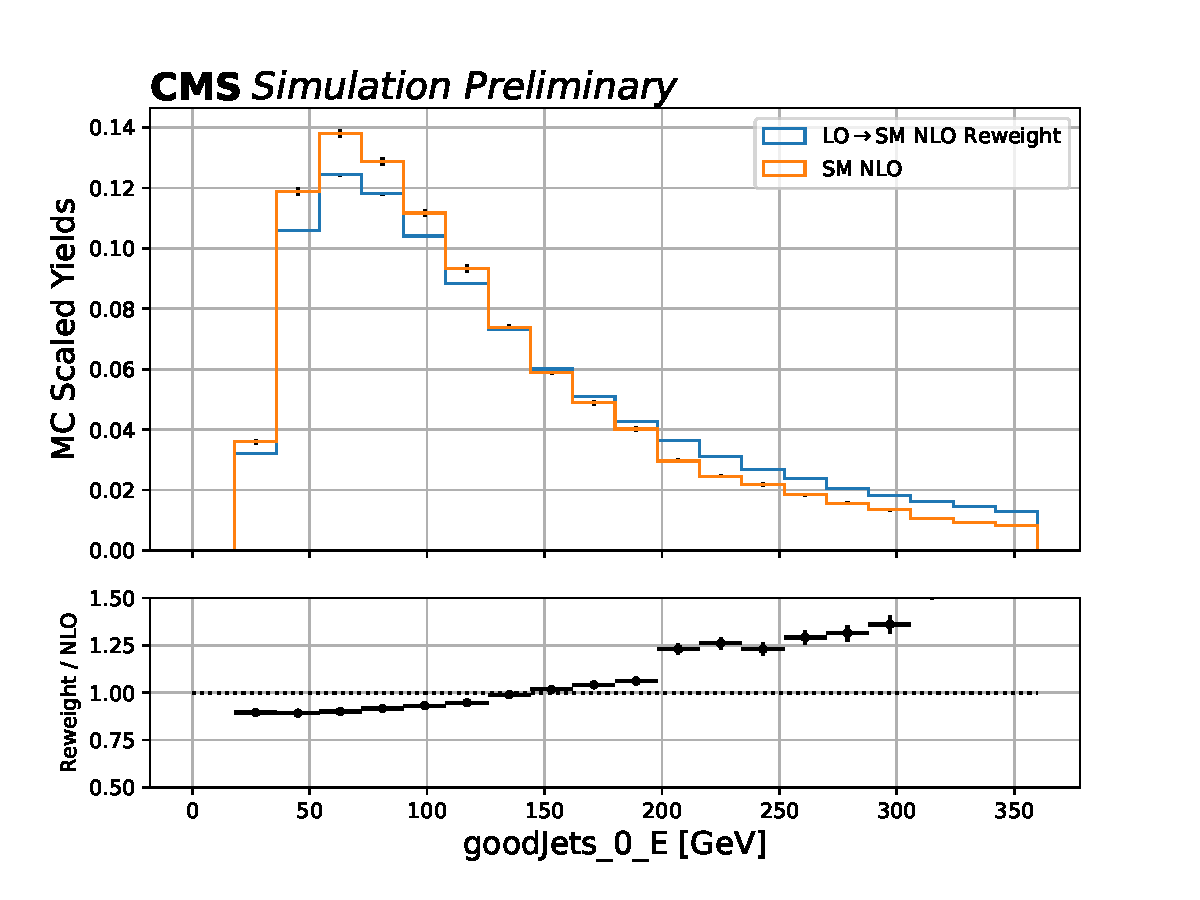
\includegraphics[width=0.4\textwidth]{Sections/HHWWgg/images/DNN/LO_NLO_Reweight_Distributions/goodJets_0_E.pdf}}
    \qquad
    \subfloat[Subleading Jet Energy]{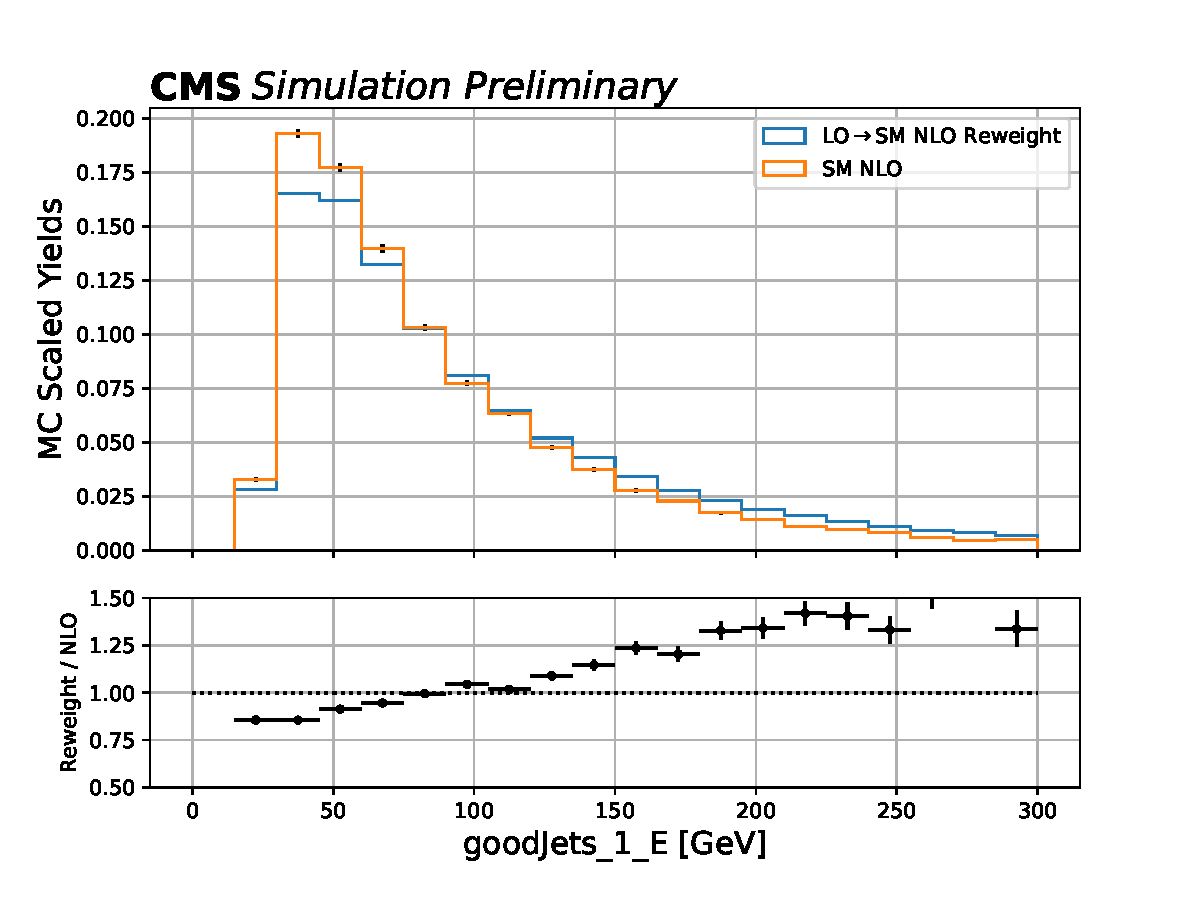
\includegraphics[width=0.4\textwidth]{Sections/HHWWgg/images/DNN/LO_NLO_Reweight_Distributions/goodJets_1_E.pdf}}
    \caption{Leading and subleading jet energy}
\end{figure}  

\newpage 

\begin{figure}[h!]
    \setcounter{subfigure}{0}
    \centering
    \subfloat[Subleading Jet $p_{T}$]{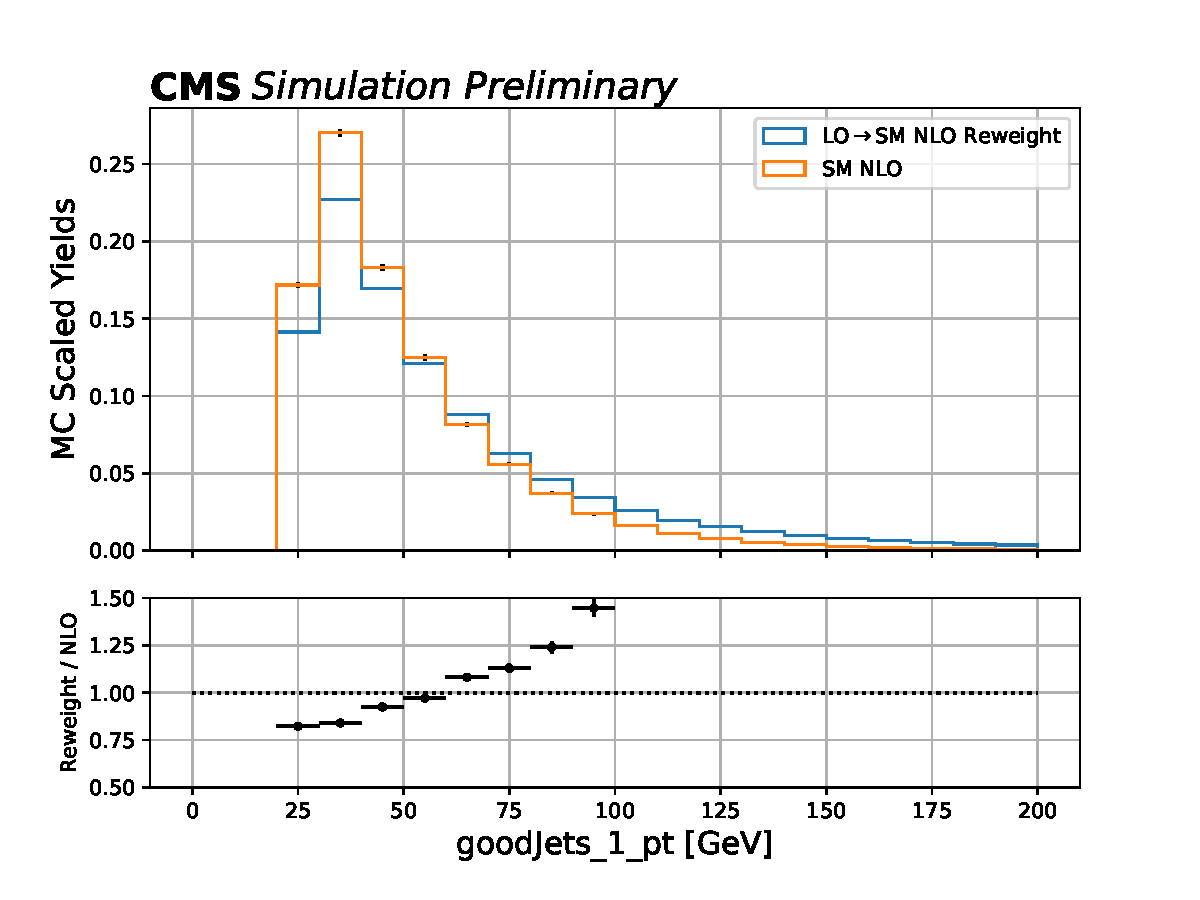
\includegraphics[width=0.4\textwidth]{Sections/HHWWgg/images/DNN/LO_NLO_Reweight_Distributions/goodJets_1_pt.pdf}}
    \qquad
    \subfloat[Lepton Energy]{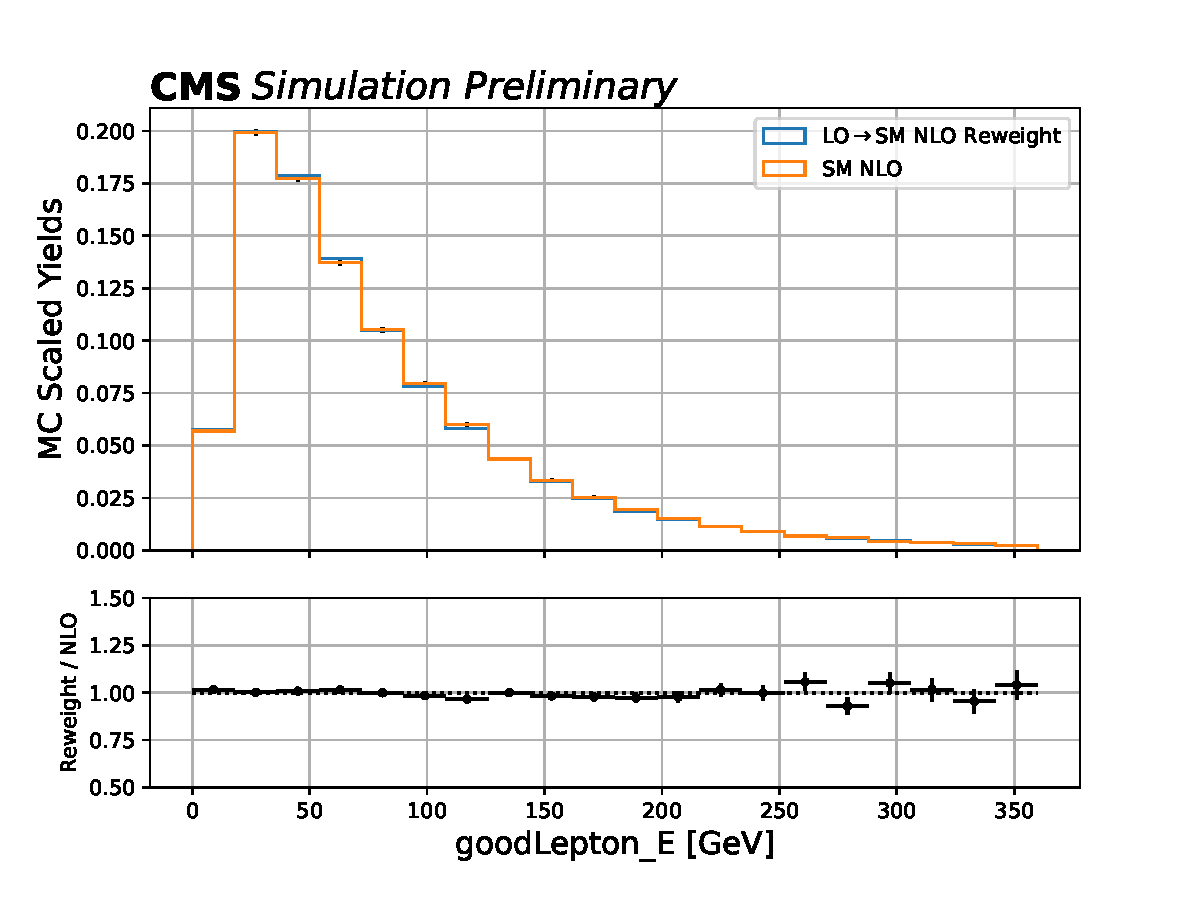
\includegraphics[width=0.4\textwidth]{Sections/HHWWgg/images/DNN/LO_NLO_Reweight_Distributions/goodLepton_E.pdf}}
    \caption{Subleading jet \pt, lepton energy}
\end{figure}

\begin{figure}[h!]
    \setcounter{subfigure}{0}
    \centering
    \subfloat[Good Lepton $\phi$]{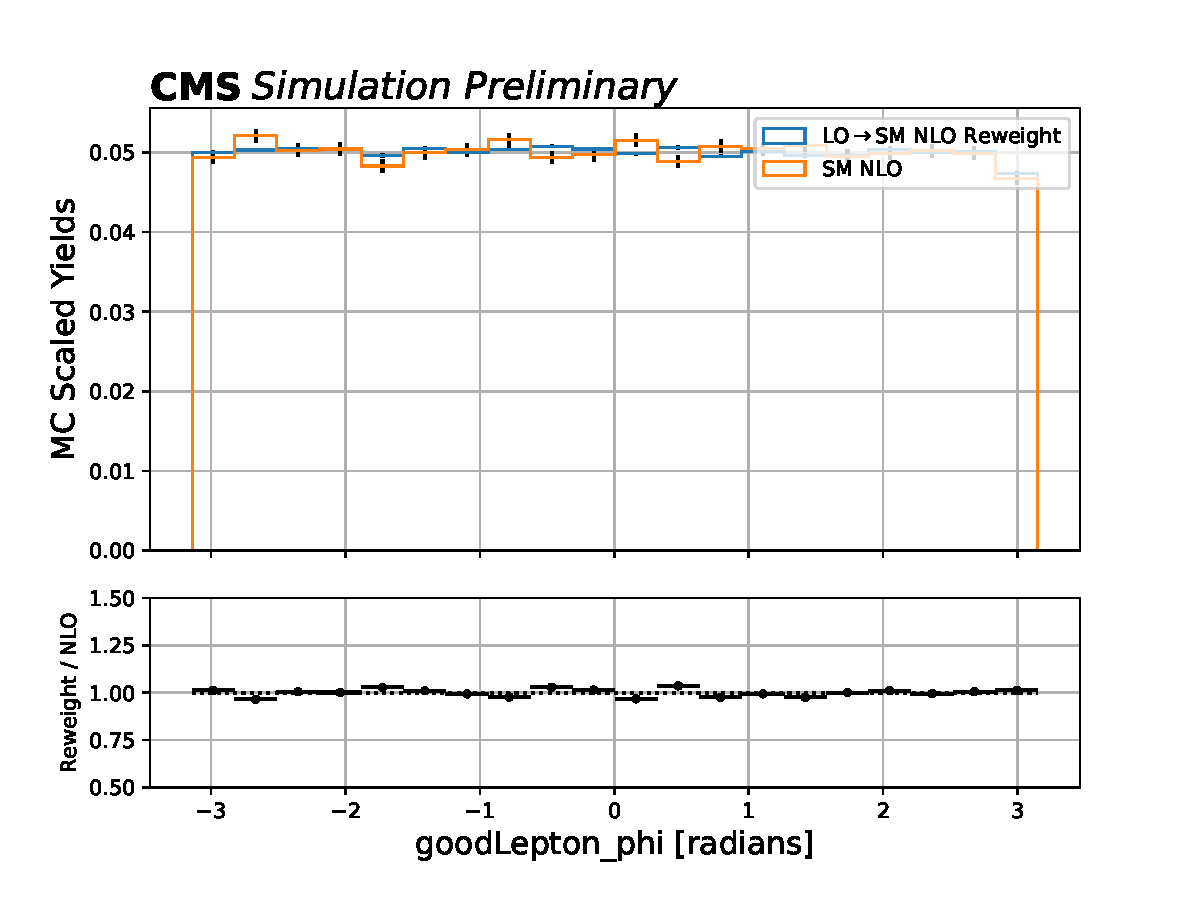
\includegraphics[width=0.4\textwidth]{Sections/HHWWgg/images/DNN/LO_NLO_Reweight_Distributions/goodLepton_phi.pdf}}
    \qquad
    \subfloat[Leading Photon MVA]{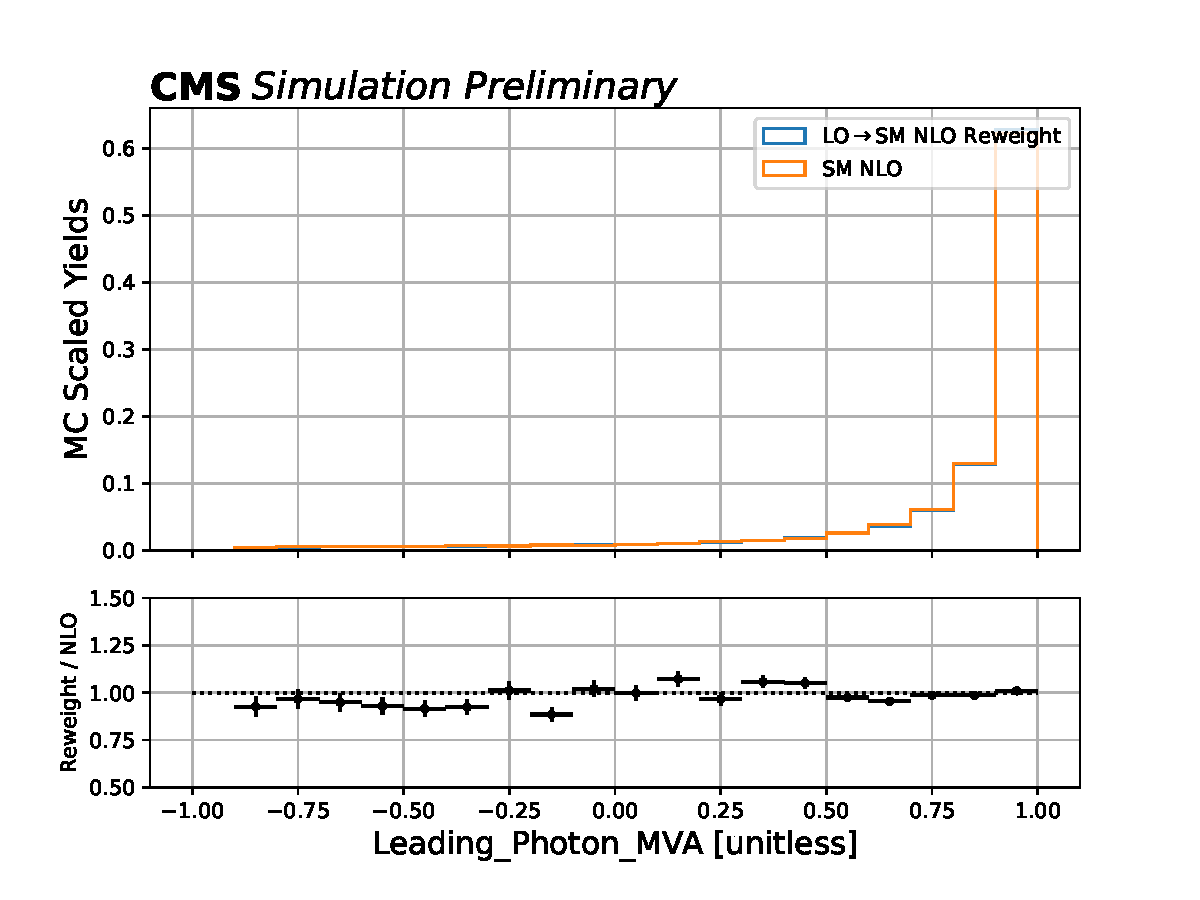
\includegraphics[width=0.4\textwidth]{Sections/HHWWgg/images/DNN/LO_NLO_Reweight_Distributions/Leading_Photon_MVA.pdf}}
    \caption{Lepton $\phi$, leading photon MVA}
\end{figure}

\newpage 

\begin{figure}[h!]
    \setcounter{subfigure}{0}
    \centering
    \subfloat[Good Lepton $\eta$]{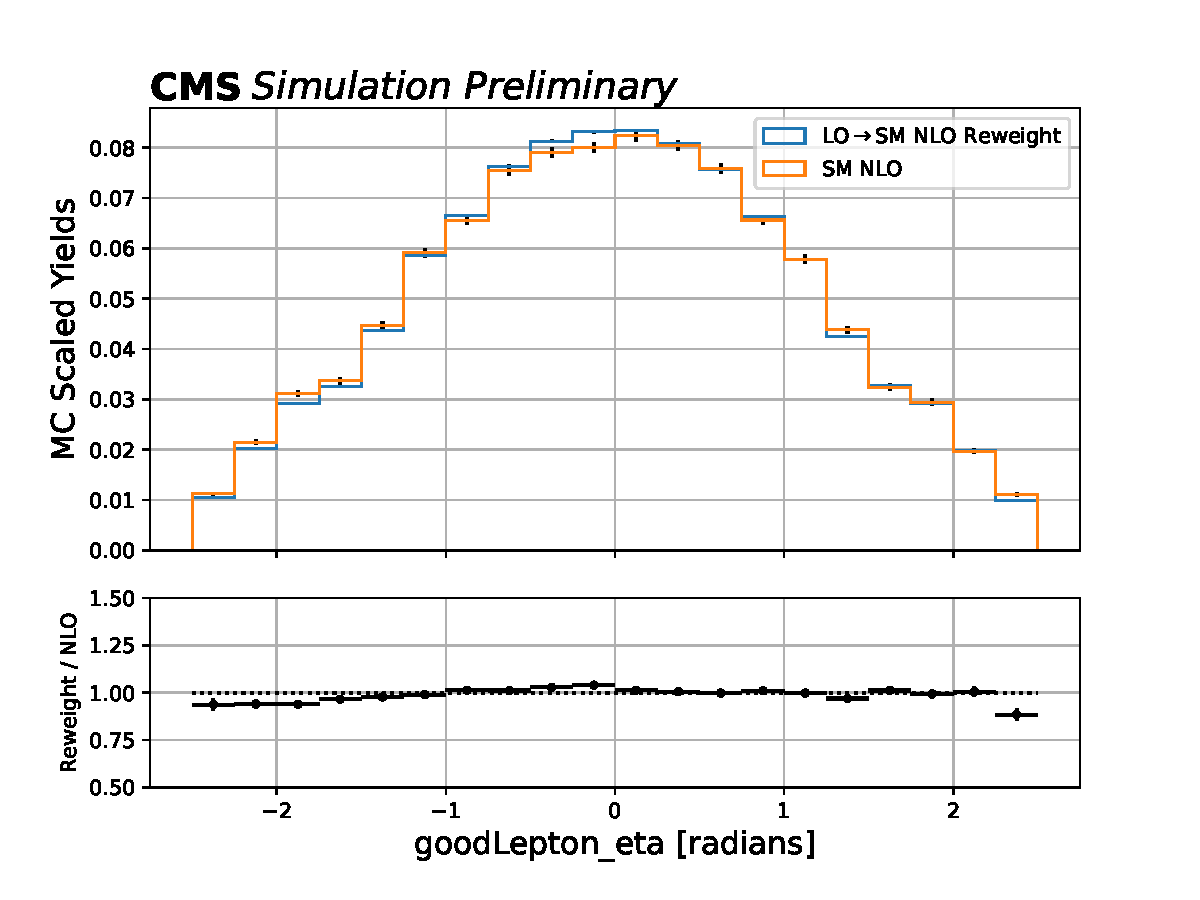
\includegraphics[width=0.4\textwidth]{Sections/HHWWgg/images/DNN/LO_NLO_Reweight_Distributions/goodLepton_eta.pdf}}
    \qquad
    \subfloat[Subleading Jet $\eta$]{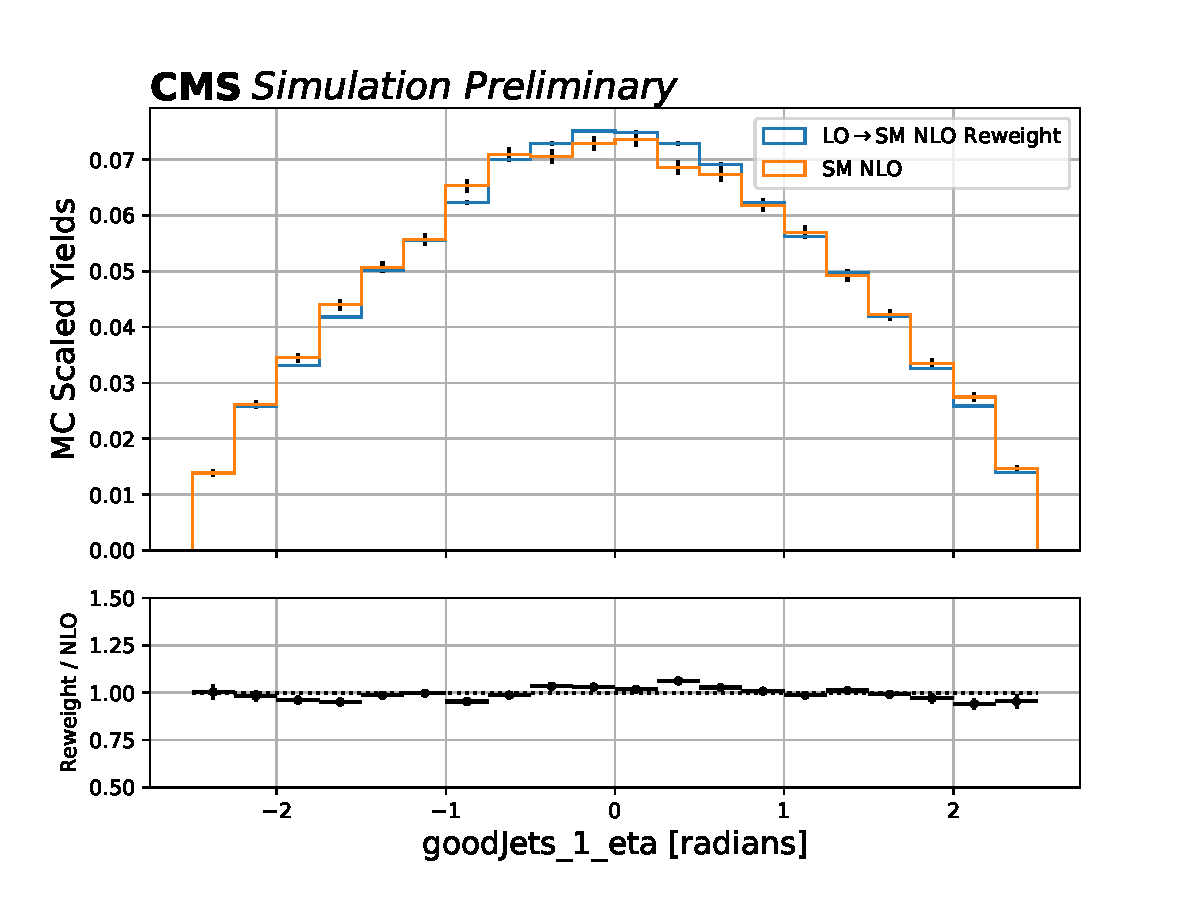
\includegraphics[width=0.4\textwidth]{Sections/HHWWgg/images/DNN/LO_NLO_Reweight_Distributions/goodJets_1_eta.pdf}}
    \caption{Lepton $\eta$, subleading jet $\eta$}
\end{figure}


\begin{figure}[h!]
    \setcounter{subfigure}{0}
    \centering
    \subfloat[Subleading Jet $\phi$]{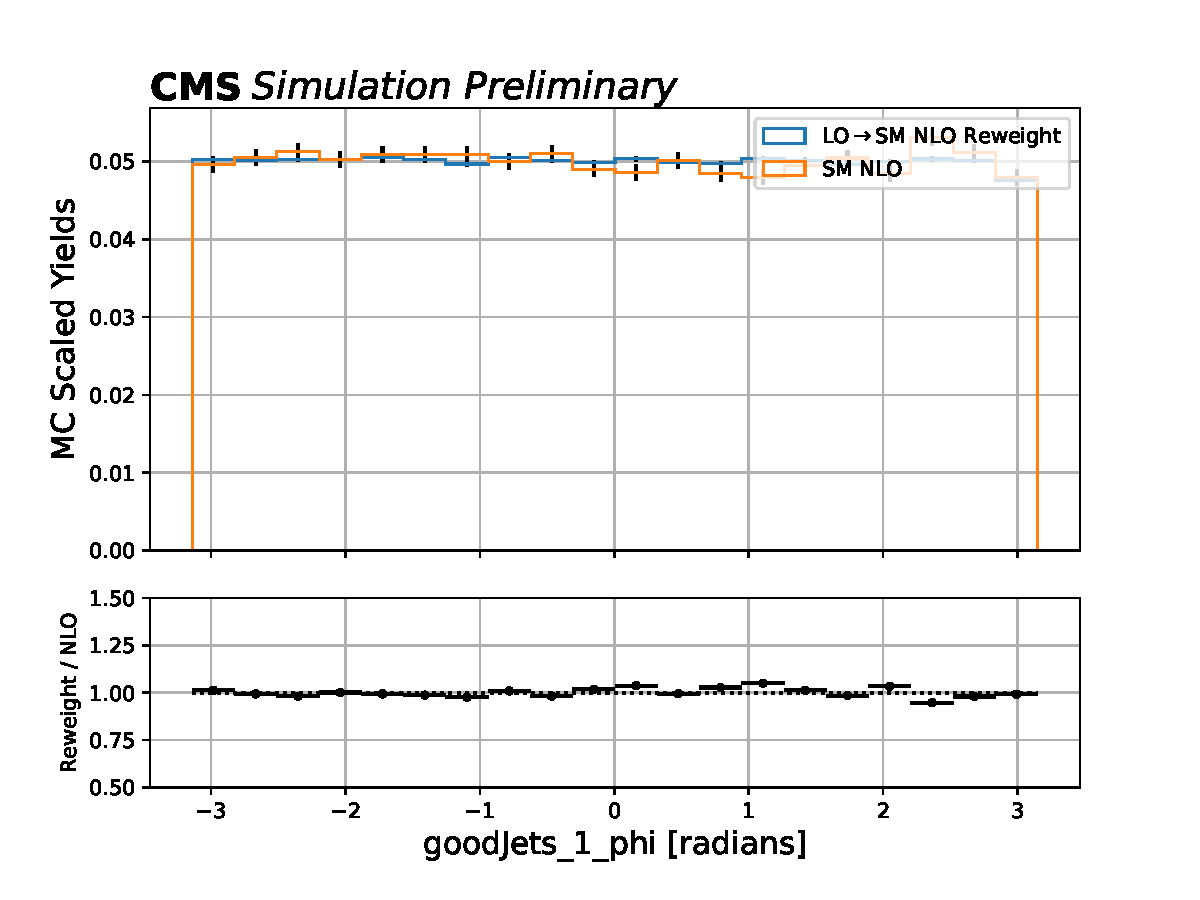
\includegraphics[width=0.4\textwidth]{Sections/HHWWgg/images/DNN/LO_NLO_Reweight_Distributions/goodJets_1_phi.pdf}}
    \qquad
    \subfloat[Subleading Photon $\eta$]{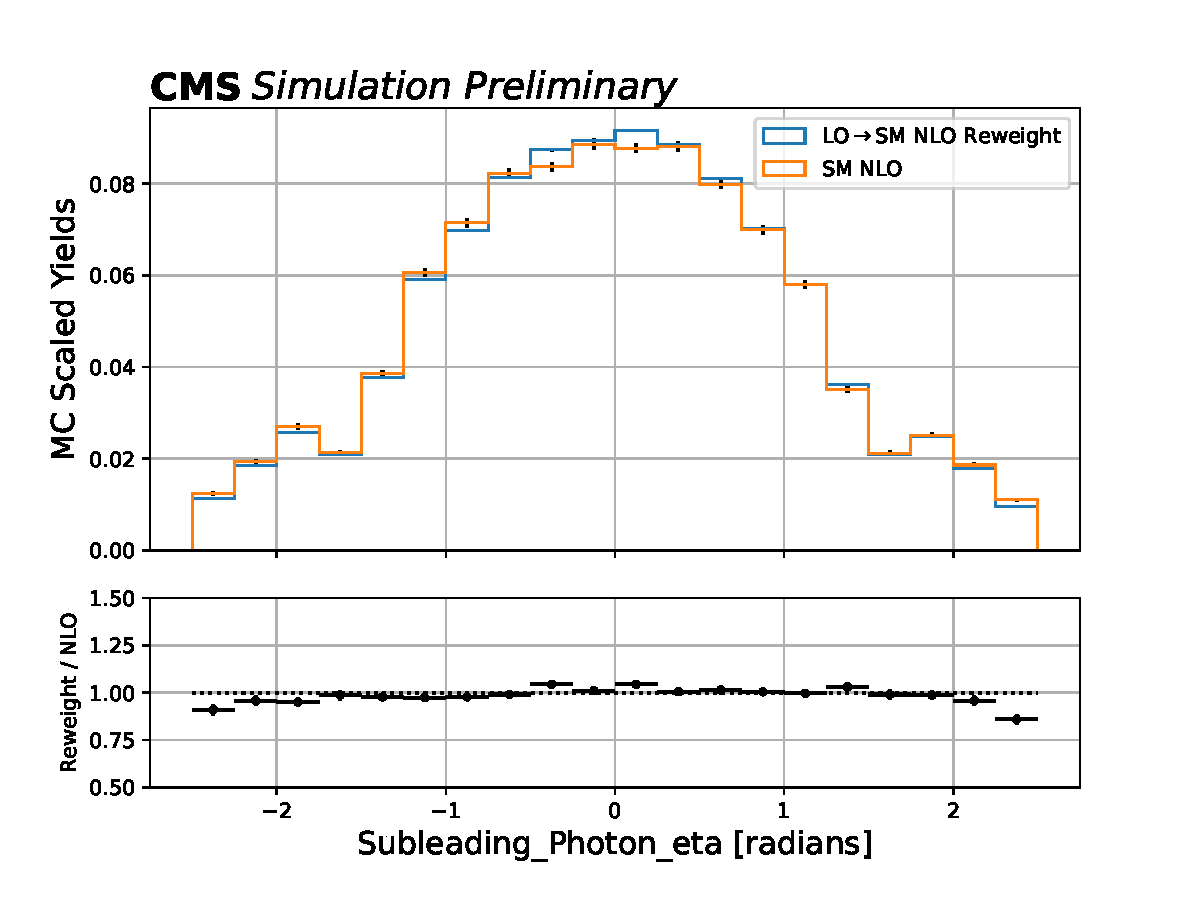
\includegraphics[width=0.4\textwidth]{Sections/HHWWgg/images/DNN/LO_NLO_Reweight_Distributions/Subleading_Photon_eta.pdf}}
    \caption{Subleading jet $\phi$, subleading photon $\eta$}
\end{figure}

\begin{figure}[h!]
    \setcounter{subfigure}{0}
    \centering
    \subfloat[Leading Jet b-tagging score]{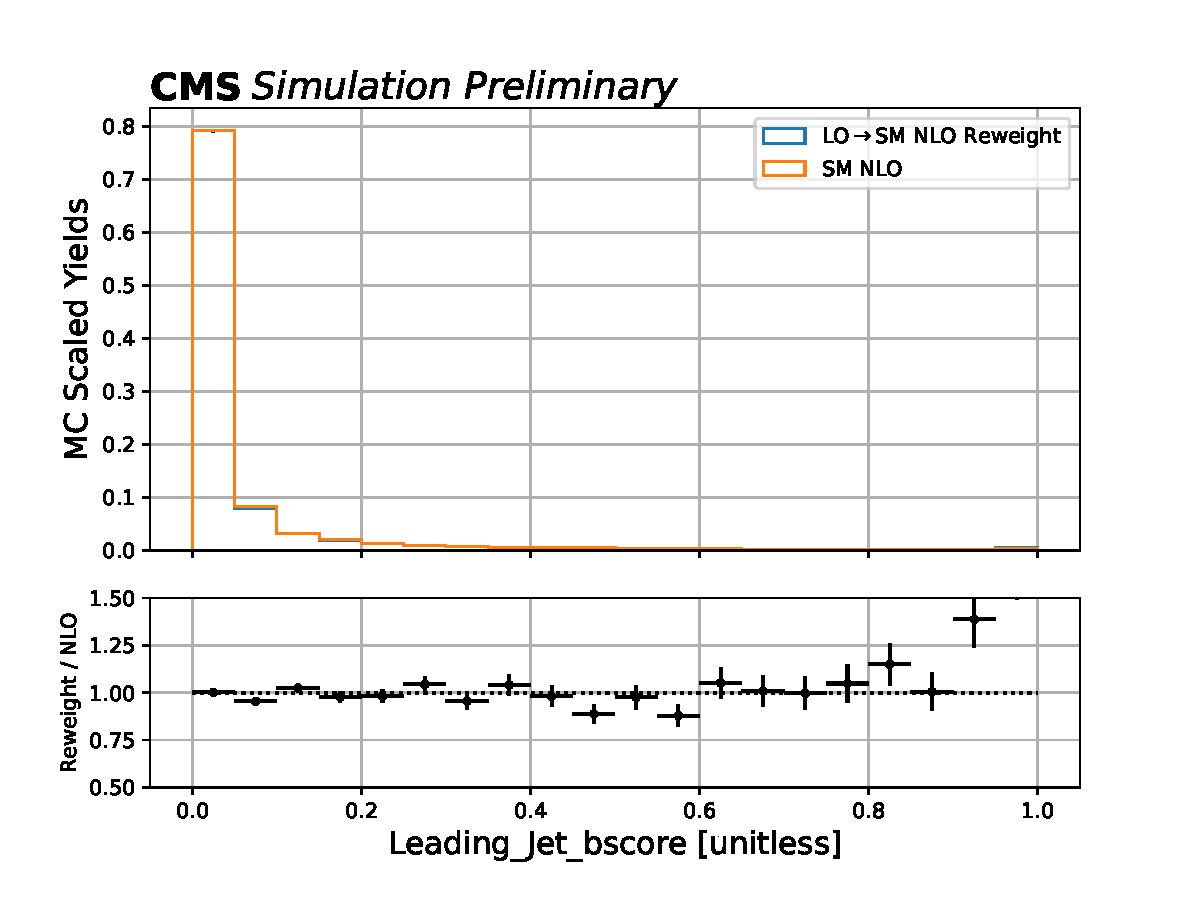
\includegraphics[width=0.4\textwidth]{Sections/HHWWgg/images/DNN/LO_NLO_Reweight_Distributions/Leading_Jet_bscore.pdf}}
    \qquad
    \subfloat[Subleading Jet b-tagging score]{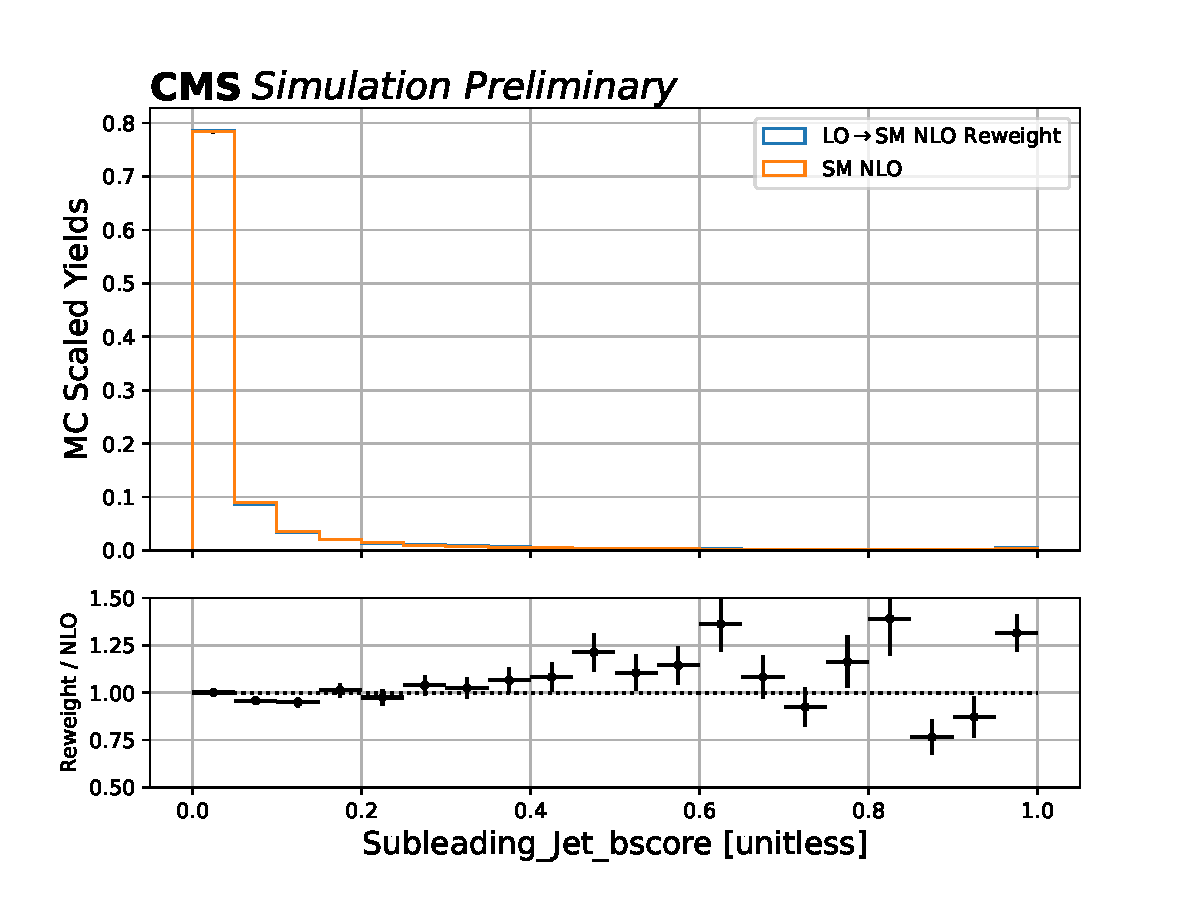
\includegraphics[width=0.4\textwidth]{Sections/HHWWgg/images/DNN/LO_NLO_Reweight_Distributions/Subleading_Jet_bscore.pdf}}
    \caption{Leading and subleading jet b-tagging score}
\end{figure}

\newpage

\begin{figure}[h!]
    \setcounter{subfigure}{0}
    \centering
    \subfloat[Subleading Photon $\phi$]{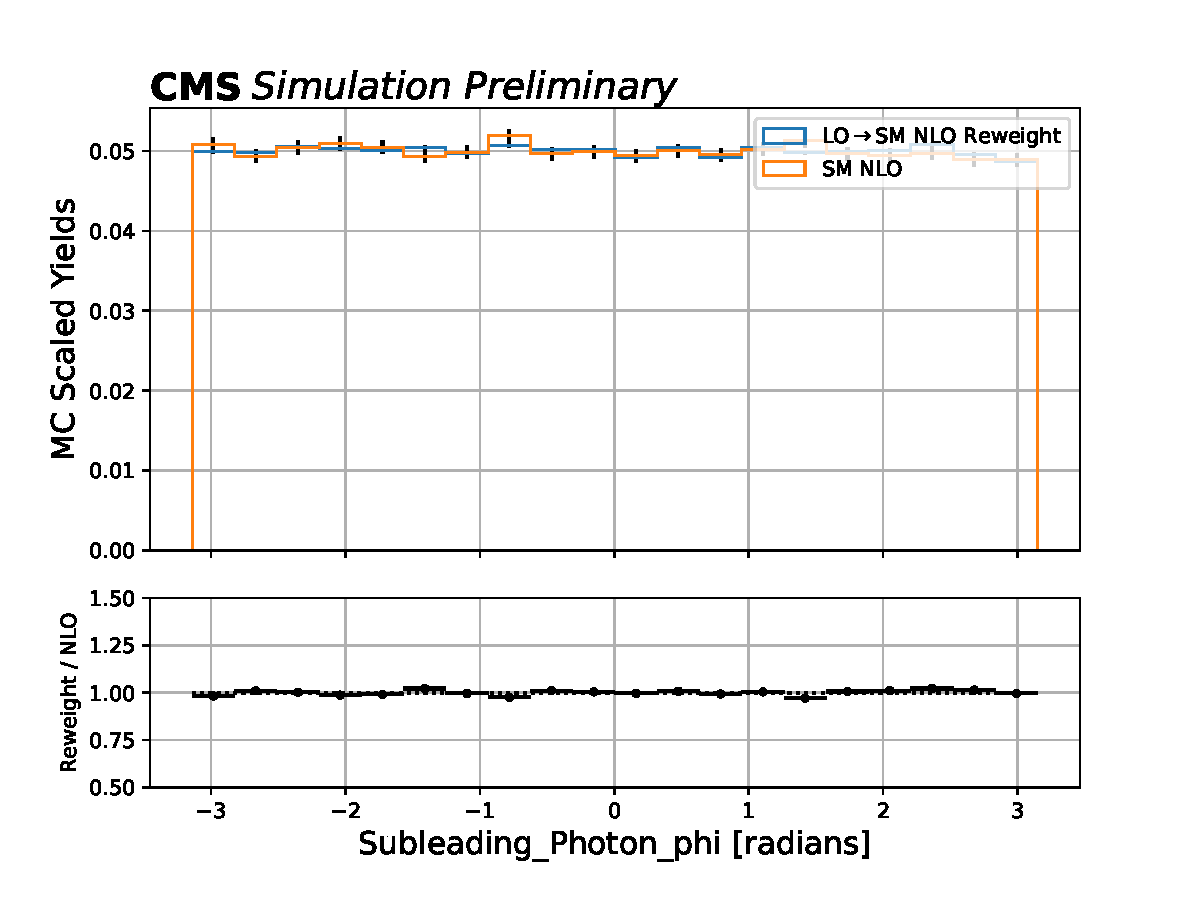
\includegraphics[width=0.4\textwidth]{Sections/HHWWgg/images/DNN/LO_NLO_Reweight_Distributions/Subleading_Photon_phi.pdf}}
    \qquad
    \subfloat[Number of jets]{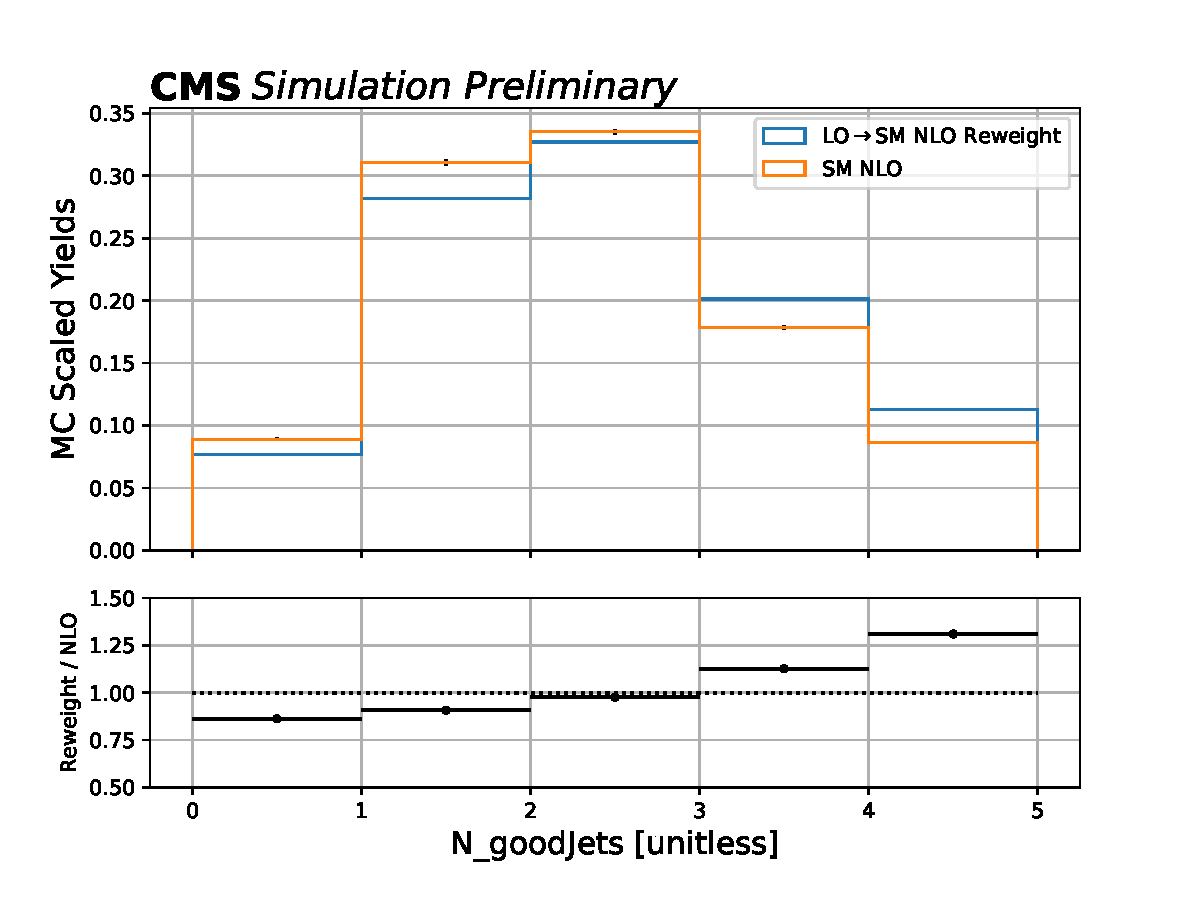
\includegraphics[width=0.4\textwidth]{Sections/HHWWgg/images/DNN/LO_NLO_Reweight_Distributions/N_goodJets.pdf}}
    \caption{Subleading photon $\phi$, number of jets}
\end{figure}

\begin{figure}[h!]
    \setcounter{subfigure}{0}
    \centering
    \subfloat[Leading Jet $\phi$]{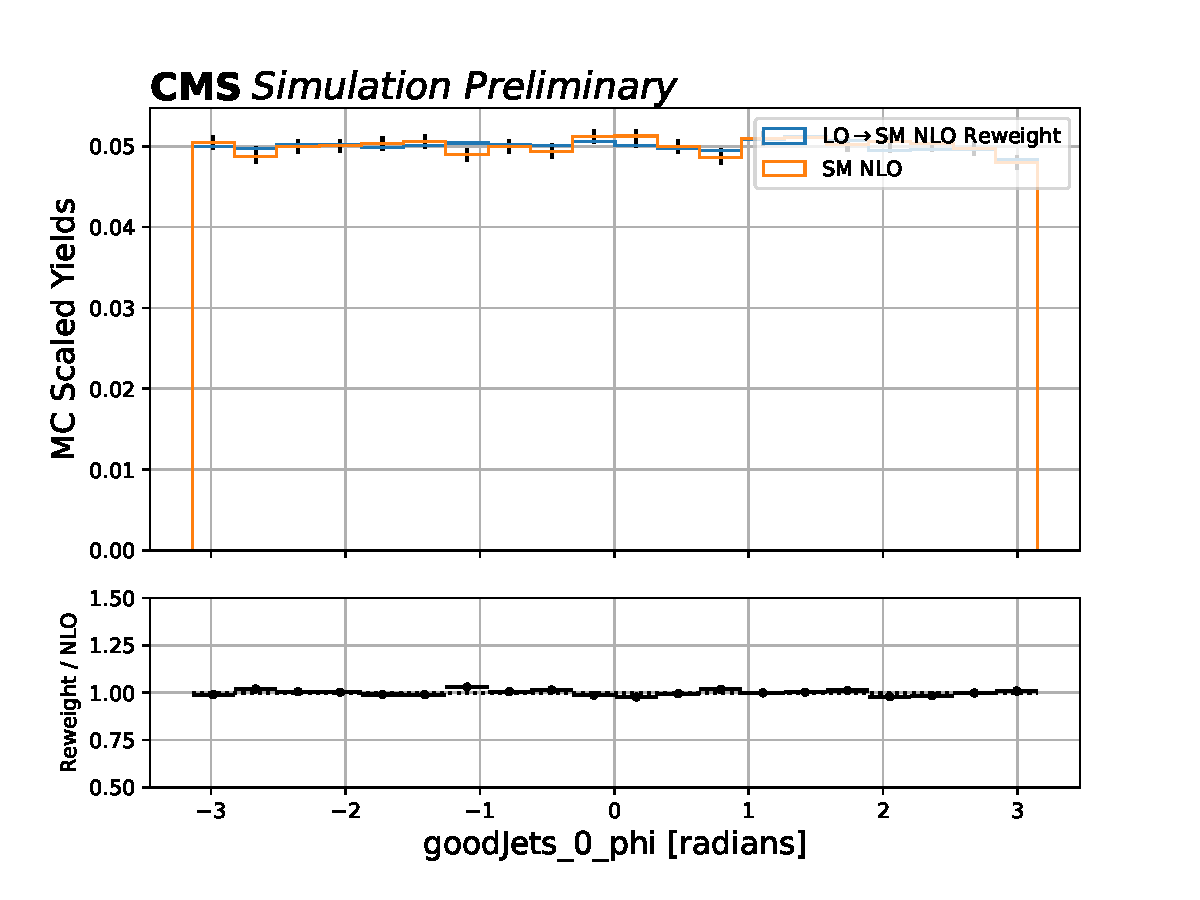
\includegraphics[width=0.4\textwidth]{Sections/HHWWgg/images/DNN/LO_NLO_Reweight_Distributions/goodJets_0_phi.pdf}}
    \qquad
    \subfloat[Scaling Leading Photon E]{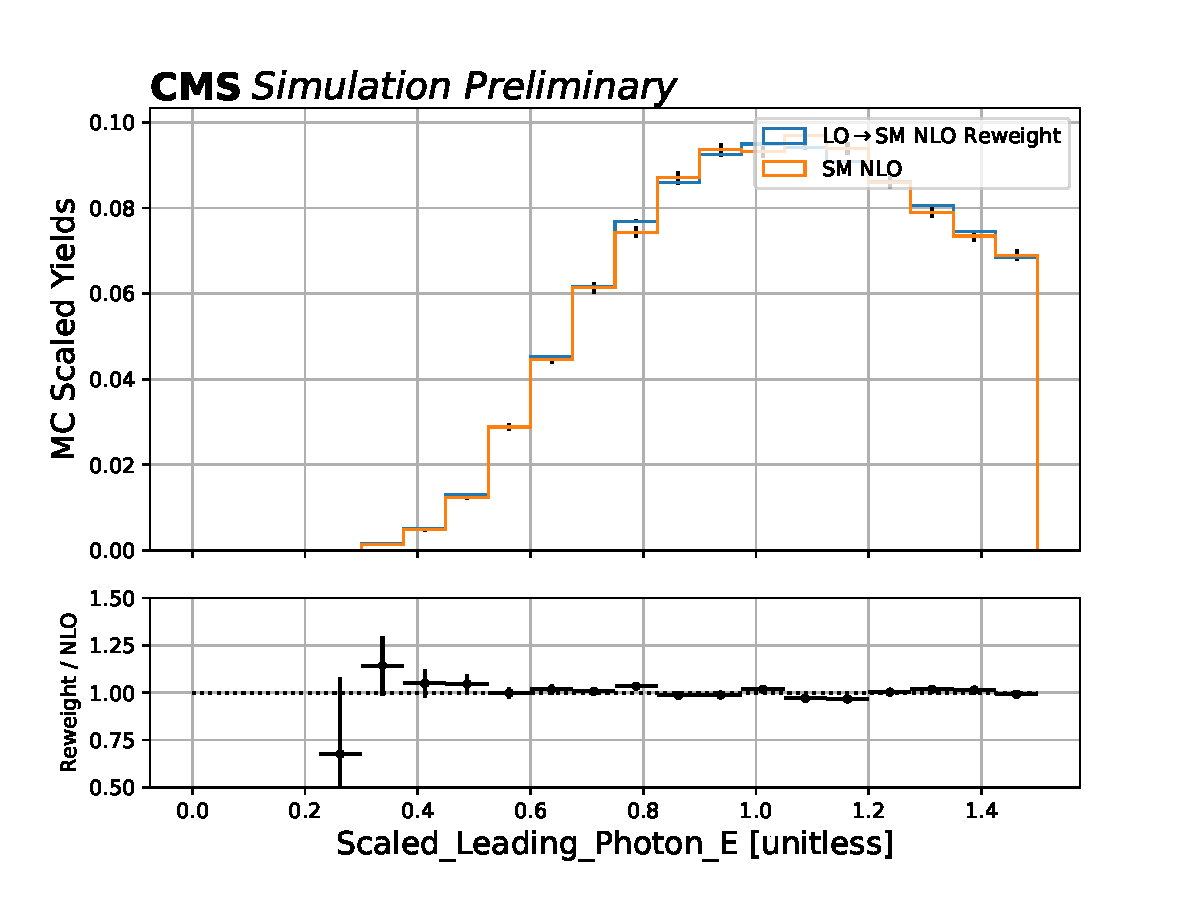
\includegraphics[width=0.4\textwidth]{Sections/HHWWgg/images/DNN/LO_NLO_Reweight_Distributions/Scaled_Leading_Photon_E.pdf}}
    \caption{Leading jet $\phi$, leading photon energy over \mgg}
\end{figure}

\begin{figure}[h!]
    \setcounter{subfigure}{0}
    \centering
    \subfloat[Subleading Photon MVA]{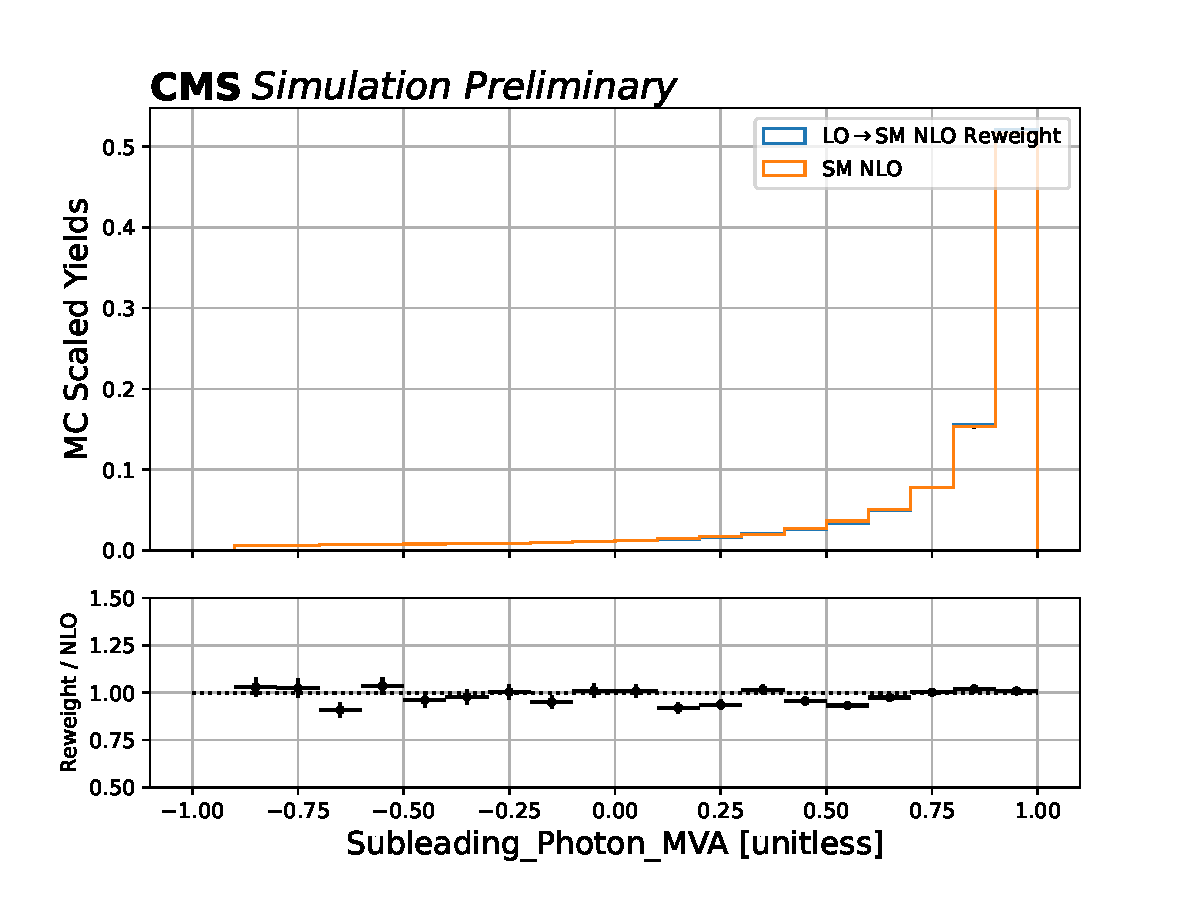
\includegraphics[width=0.4\textwidth]{Sections/HHWWgg/images/DNN/LO_NLO_Reweight_Distributions/Subleading_Photon_MVA.pdf}}
    \qquad
    \subfloat[Leading Jet $\eta$]{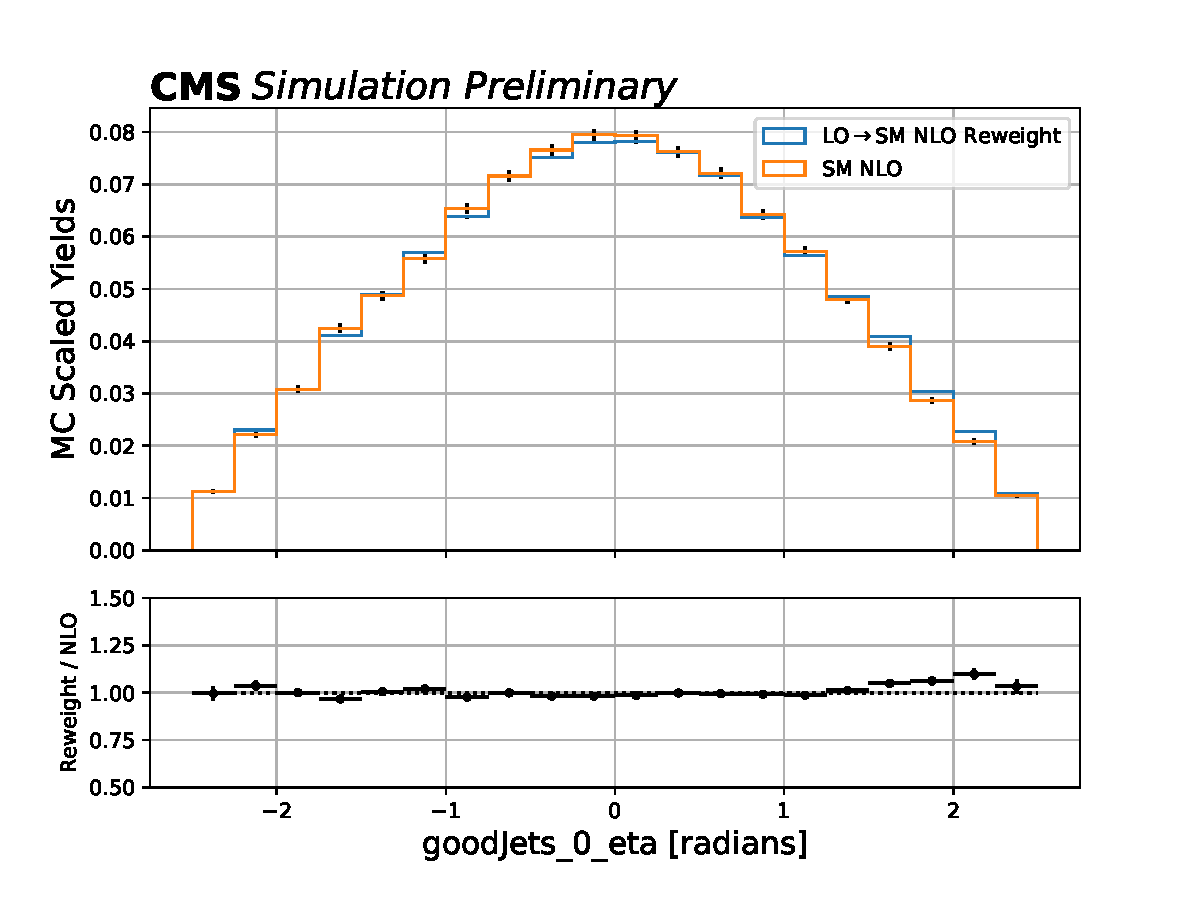
\includegraphics[width=0.4\textwidth]{Sections/HHWWgg/images/DNN/LO_NLO_Reweight_Distributions/goodJets_0_eta.pdf}}
    \caption{Subleading photon MVA, leading jet $\eta$}
\end{figure}

\newpage 

\begin{figure}[h!]
    \setcounter{subfigure}{0}
    \centering
    \subfloat[Leading Photon $\eta$]{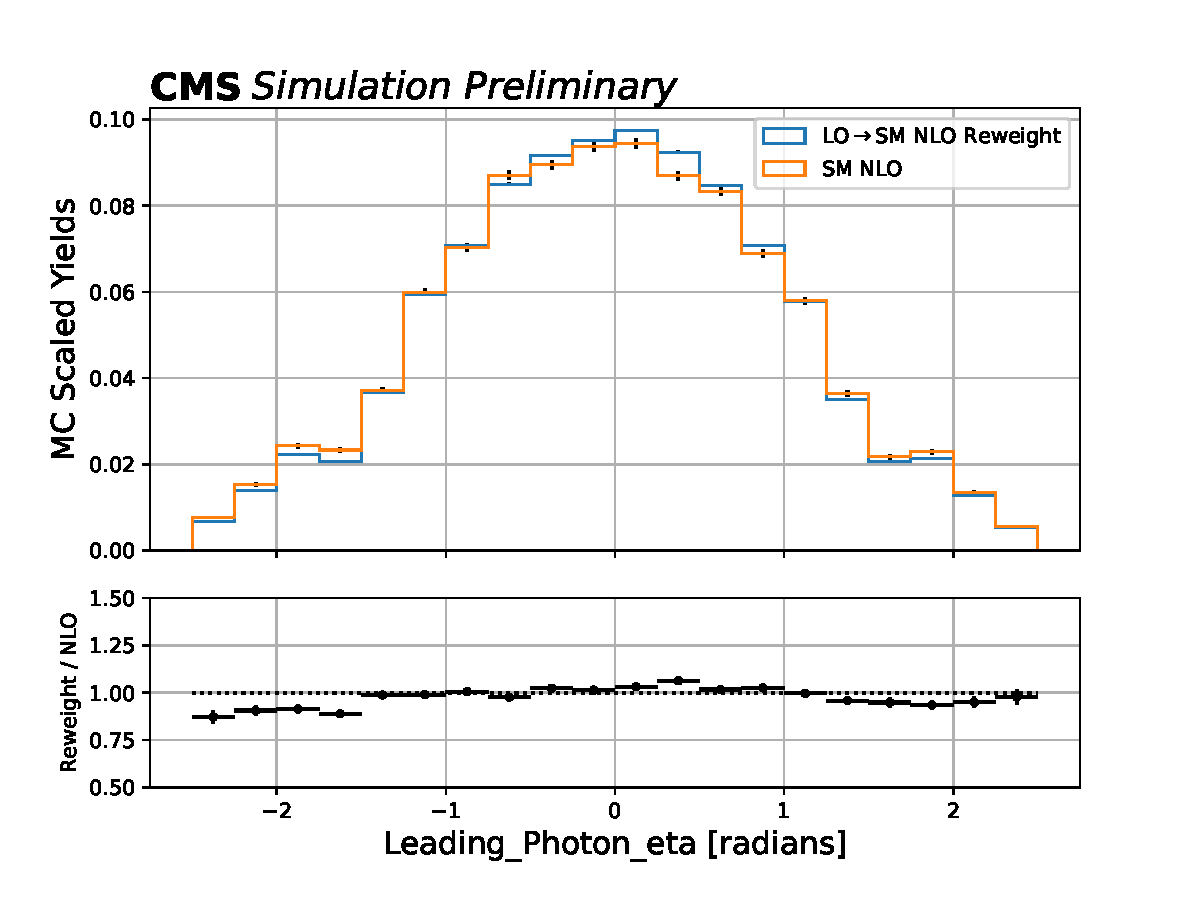
\includegraphics[width=0.4\textwidth]{Sections/HHWWgg/images/DNN/LO_NLO_Reweight_Distributions/Leading_Photon_eta.pdf}}
    \qquad
    \subfloat[Transverse Mass of lepton and MET]{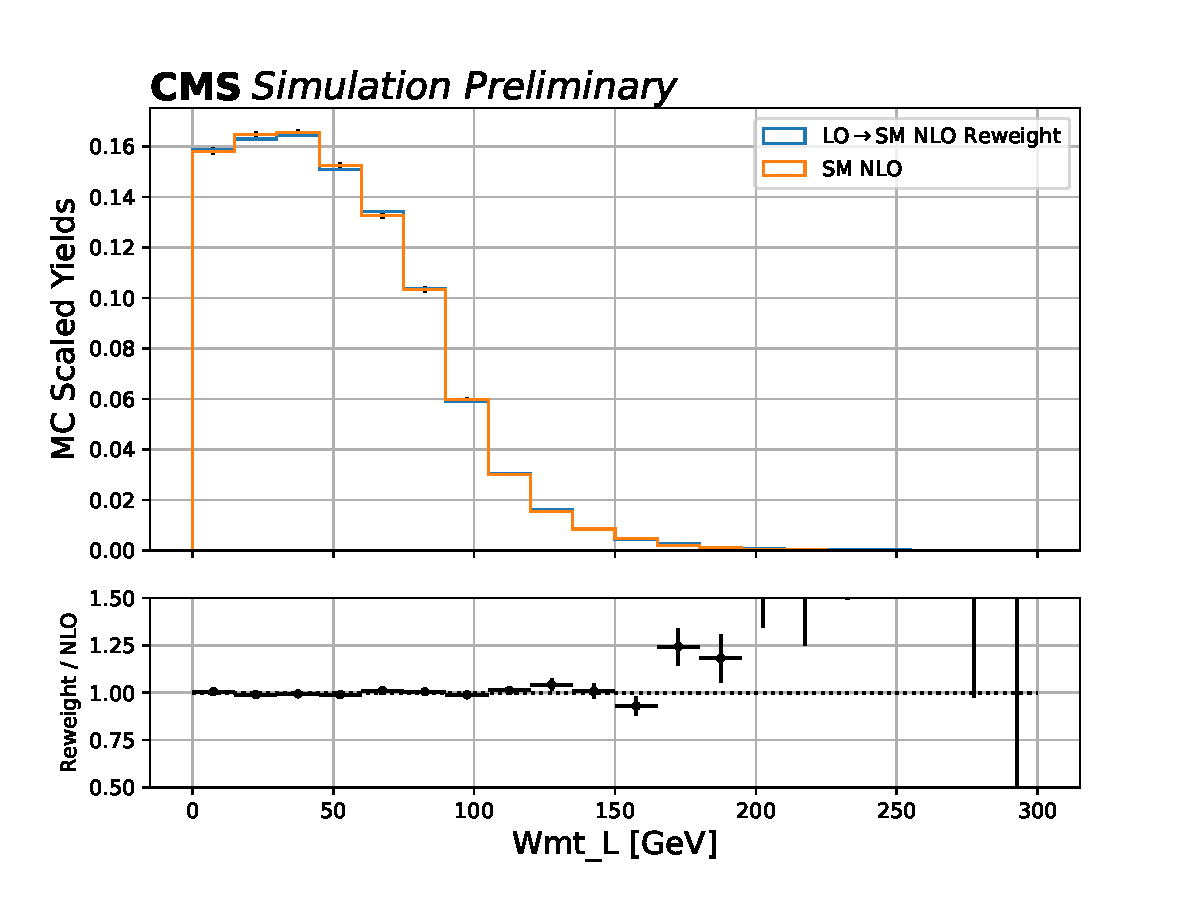
\includegraphics[width=0.4\textwidth]{Sections/HHWWgg/images/DNN/LO_NLO_Reweight_Distributions/Wmt_L.pdf}}
    \caption{Leading photon $\eta$, transverse W mass}
\end{figure}

